
%% $Id$

\documentclass[12pt,a4paper]{report}
\usepackage{latexsym}
\usepackage{amssymb}
\usepackage[english]{babel}
\usepackage[latin1]{inputenc}
\usepackage[only,bigsqcap]{stmaryrd}
\usepackage{wasysym}
\usepackage{eufrak}
\usepackage{textcomp}
\usepackage{marvosym}
\usepackage{supertabular}
\let\intorig=\int  %iman.sty redefines \int
\usepackage{graphicx,../iman,../extra,../ttbox,../../Distribution/lib/texinputs/isabelle,../../Distribution/lib/texinputs/isabellesym,../pdfsetup}

\isabellestyle{it}

\title{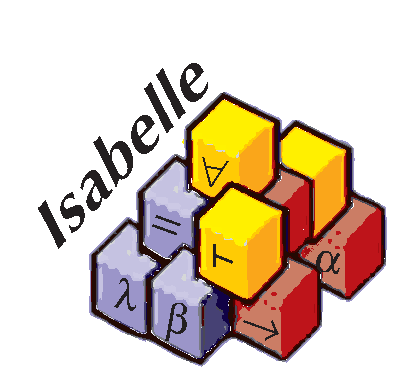
\includegraphics[scale=0.5]{isabelle} \\[4ex] The Isabelle System Manual}

\author{\emph{Markus Wenzel} and \emph{Stefan Berghofer} \\
  TU M\"unchen}

\makeindex

\setcounter{secnumdepth}{1} \setcounter{tocdepth}{2}

\pagestyle{headings}
\sloppy
\binperiod     %%%treat . like a binary operator

\begin{document}

\underscoreoff

\maketitle 
\pagenumbering{roman} \tableofcontents \clearfirst


% $Id$

\chapter{The Isabelle system environment}

This manual describes Isabelle together with related tools and user interfaces
as seen from an outside (system oriented) view.  See also the \emph{Isabelle
  Reference Manual}~\cite{isabelle-ref} and the \emph{Isabelle Isar Reference
  Manual}~\cite{isabelle-isar-ref} for the actual Isabelle commands and
related functions.

\medskip The Isabelle system environment is based on a few general elements:
\begin{itemize}
\item The \emph{Isabelle settings mechanism}, which provides environment
  variables to all Isabelle programs (including tools and user interfaces).
\item \emph{Isabelle proper} (\ttindex{isabelle}), which invokes logic
  sessions, both interactively or in batch mode. In particular,
  \texttt{isabelle} abstracts over the invocation of the actual {\ML} system
  to be used.
\item The \emph{Isabelle tools wrapper} (\ttindex{isatool}), which provides a
  generic startup platform for Isabelle related utilities.  Thus tools
  automatically benefit from the settings mechanism.
\item The \emph{Isabelle interface wrapper} (\ttindex{Isabelle}\footnote{Note
    the capital \texttt{I}!}), which provides some abstraction over the actual
  user interface to be used.
\end{itemize}

\medskip The beginning user would probably just run one of the interfaces (by
invoking the capital \texttt{Isabelle}), and maybe some basic tools like
\texttt{doc} (see \S\ref{sec:tool-doc}).  This assumes that the system has
already been installed, of course.\footnote{In case you have to do this
  yourself, see the \ttindex{INSTALL} file in the top-level directory of the
  distribution of how to proceed.  Some binary packages are available as
  well.}


\section{Isabelle settings} \label{sec:settings}

The Isabelle system heavily depends on the \emph{settings
  mechanism}\indexbold{settings}. Basically, this is a statically scoped
collection of environment variables, such as \texttt{ISABELLE_HOME},
\texttt{ML_SYSTEM}, \texttt{ML_HOME}.  These variables are \emph{not} intended
to be set directly from the shell, though.  Isabelle employs a somewhat more
sophisticated scheme of \emph{settings files} --- one for site-wide defaults,
another for additional user-specific modifications.  With all configuration
variables in at most two places, this scheme is more maintainable and
user-friendly than plain shell environment variables.

In particular, we avoid the typical situation where prospective users of a
software package are told to put several things into their shell startup
scripts, before being able to actually run the program. Isabelle requires none
such administrative chores of its end-users --- the executables can be invoked
straight away.\footnote{Occasionally, users would still want to put the
  Isabelle \texttt{bin} directory into their shell's search path, but this is
  not required.}


\subsection{Building the environment}

Whenever any of the Isabelle executables is run, their settings environment is
built as follows.

\begin{enumerate}
\item The special variable \settdx{ISABELLE_HOME} is determined automatically
  from the location of the binary that has been run.
  
  You should not try to set \texttt{ISABELLE_HOME} manually. Also note that
  the Isabelle executables either have to be run from their original location
  in the distribution directory, or via the executable objects created by the
  \texttt{install} utility (see \S\ref{sec:tool-install}).  Just doing a plain
  copy of the \texttt{bin} files will not work!
  
\item The file \texttt{\$ISABELLE_HOME/etc/settings} ist run as a shell script
  with the auto-export option for variables enabled.
  
  This file typically contains a rather long list of shell variable
  assigments, thus providing the site-wide default settings.  The Isabelle
  distribution already contains a global settings file with sensible defaults
  for most variables. When installing the system, only a few of these have to
  be adapted (most likely \texttt{ML_SYSTEM} etc.).
  
\item The file \texttt{\$ISABELLE_HOME_USER/etc/settings} (if it exists) is
  run in the same way as the site default settings. Note that the variable
  \texttt{ISABELLE_HOME_USER} has already been set before --- usually to
  \texttt{\~\relax/isabelle}.
  
  Thus individual users may override the site-wide defaults. See also file
  \texttt{etc/user-settings.sample} in the distribution.  Typically, a user
  settings file would contain only a few lines, just the assigments that are
  really changed.  One should definitely \emph{not} start with a full copy the
  basic \texttt{\$ISABELLE_HOME/etc/settings}. This could cause very annoying
  maintainance problems later, when the Isabelle installation is updated or
  changed otherwise.

\end{enumerate}

Note that settings files are actually full GNU bash scripts. So one may use
complex shell commands, such as \texttt{if} or \texttt{case} statements to set
variables depending on the system architecture or other environment variables.
Such advanced features should be added only with great care, though. In
particular, external environment references should be kept at a minimum.

\medskip A few variables are somewhat special:
\begin{itemize}
\item \settdx{ISABELLE} and \settdx{ISATOOL} are set automatically to
  the absolute path names of the \texttt{isabelle} and
  \texttt{isatool} executables, respectively.
  
\item \settdx{ISABELLE_OUTPUT} will has the {\ML} system identifier (according
  to \texttt{ML_IDENTIFIER}) automatically appended to its value.
\end{itemize}

\medskip The Isabelle settings scheme is basically simple, but non-trivial.
For debugging purposes, the resulting environment may be inspected with the
\texttt{getenv} utility, see \S\ref{sec:tool-getenv}.


\subsection{Common variables}

This is a reference of common Isabelle settings variables. Note that the list
is somewhat open-ended. Third-party utilities or interfaces may add their own
selection. Variables that are special in some sense are marked with *.

\begin{description}
\item[\settdx{ISABELLE_HOME}*] is the location of the top-level Isabelle
  distribution directory. This is automatically determined from the Isabelle
  executable that has been invoked.  Do not try to set \texttt{ISABELLE_HOME}
  yourself from the shell.
  
\item[\settdx{ISABELLE_HOME_USER}] is the user-specific counterpart of
  \texttt{ISABELLE_HOME}. The default value is \texttt{\~\relax/isabelle},
  under rare circumstances this may be changed in the global setting file.
  Typically, the \texttt{ISABELLE_HOME_USER} directory mimics
  \texttt{ISABELLE_HOME} to some extend. In particular, site-wide defaults may
  be overridden by a private \texttt{etc/settings}.
  
\item[\settdx{ISABELLE}*, \settdx{ISATOOL}*] are automatically set to the full
  path names of the \texttt{isabelle} and \texttt{isatool} executables,
  respectively.  Thus other tools and scripts need not assume that the
  Isabelle \texttt{bin} directory is on the current search path of the shell.
  
\item[\settdx{ML_SYSTEM}, \settdx{ML_HOME}, \settdx{ML_OPTIONS},
  \settdx{ML_PLATFORM}, \settdx{ML_IDENTIFIER}*] specify the underlying {\ML}
  system to be used for Isabelle.  There is only a fixed set of admissable
  \texttt{ML_SYSTEM} names (see the \texttt{etc/settings} file of the
  distribution).
  
  The actual compiler binary will be run from the directory \texttt{ML_HOME},
  with \texttt{ML_OPTIONS} as first arguments on the command line.  The
  optional \texttt{ML_PLATFORM} may specify the binary format of ML heap
  images, which is useful for cross-platform installations.  The value of
  \texttt{ML_IDENTIFIER} is automatically obtained by composing the
  \texttt{ML_SYSTEM} and \texttt{ML_PLATFORM} values.
  
\item[\settdx{ISABELLE_PATH}] is a list of directories (separated by colons)
  where Isabelle logic images may reside.  When looking up heaps files, the
  value of \texttt{ML_IDENTIFIER} is appended to each component internally.
  
\item[\settdx{ISABELLE_OUTPUT}*] is a directory where output heap files should
  be stored by default. The \texttt{ML_SYSTEM} identifier is appended here,
  too.
  
\item[\settdx{ISABELLE_BROWSER_INFO}] is the directory where theory browser
  information (HTML text, graph data, and printable documents) is stored (see
  also \S\ref{sec:info}).  The default value is
  \texttt{\$ISABELLE_HOME_USER/browser_info}.
  
\item[\settdx{ISABELLE_LOGIC}] specifies the default logic to load if none is
  given explicitely by the user.  The default value is \texttt{HOL}.
  
\item[\settdx{ISABELLE_USEDIR_OPTIONS}] is implicitly prefixed to the command
  line of any \texttt{isatool usedir} invocation (see also
  \S\ref{sec:tool-usedir}). This typically contains compilation options for
  object-logics --- \texttt{usedir} is the basic utility for managing logic
  sessions (cf.\ the \texttt{IsaMakefile}s in the distribution).
  
\item[\settdx{ISABELLE_LATEX}, \settdx{ISABELLE_PDFLATEX},
  \settdx{ISABELLE_BIBTEX}, \settdx{ISABELLE_DVIPS}] refer to {\LaTeX} related
  tools for Isabelle document preparation (see also \S\ref{sec:tool-latex}).
  
\item[\settdx{ISABELLE_TOOLS}] is a colon separated list of directories that
  are scanned by \texttt{isatool} for external utility programs (see also
  \S\ref{sec:isatool}).
  
\item[\settdx{ISABELLE_DOCS}] is a colon separated list of directories with
  documentation files.
  
\item[\settdx{DVI_VIEWER}] specifies the command to be used for displaying
  \texttt{dvi} files.
  
\item[\settdx{ISABELLE_INSTALL_FONTS}] determines the way that the Isabelle
  symbol fonts are installed into your currently running X11 display server.
  X11 fonts are a subtle issue, see \S\ref{sec:tool-installfonts} for more
  information.
  
\item[\settdx{ISABELLE_TMP_PREFIX}] is the prefix from which any running
  \texttt{isabelle} process derives an individual directory for temporary
  files.  The default is somewhere in \texttt{/tmp}.
  
\item[\settdx{ISABELLE_INTERFACE}] is an identifier that specifies the actual
  user interface that the capital \texttt{Isabelle} should invoke.  See
  \S\ref{sec:interface} for more details.

\end{description}


\section{Isabelle proper --- \texttt{isabelle}}

The \ttindex{isabelle} executable runs bare-bones logic sessions --- either
interactively or in batch mode. It provides an abstraction over the underlying
{\ML} system, and over the actual heap file locations. Its usage is:
\begin{ttbox}
Usage: isabelle [OPTIONS] [INPUT] [OUTPUT]

  Options are:
    -C           tell ML system to copy output image
    -I           startup Isar interaction mode
    -P           startup Proof General interaction mode
    -c           tell ML system to compress output image
    -e MLTEXT    pass MLTEXT to the ML session
    -m MODE      add print mode for output
    -q           non-interactive session
    -r           open heap file read-only
    -u           pass 'use"ROOT.ML";' to the ML session
    -w           reset write permissions on OUTPUT

  INPUT (default "\$ISABELLE_LOGIC") and OUTPUT specify in/out heaps.
  These are either names to be searched in the Isabelle path, or
  actual file names (containing at least one /).
  If INPUT is "RAW_ML_SYSTEM", just start the bare bones ML system.
\end{ttbox}
Input files without path specifications are looked up in the
\texttt{ISABELLE_PATH} setting, which may consist of multiple components
separated by colons --- these are tried in the given order with the value of
\texttt{ML_IDENTIFIER} appended internally.  In a similar way, base names are
relative to the directory specified by \texttt{ISABELLE_OUTPUT}.  In any case,
actual file locations may also be given by including at least one slash
(\texttt{/}) in the name (hint: use \texttt{./} to refer to the current
directory).


\subsection*{Options}

If the input heap file does not have write permission bits set, or the
\texttt{-r} option is given explicitely, then the session started will be
read-only.  That is, the {\ML} world cannot be committed back into the logic
image.  Otherwise, a writable session enables commits into either the input
file, or into an alternative output heap file (in case that is given as the
second argument on the command line).

The read-write state of sessions is determined at startup only, it cannot be
changed intermediately. Also note that heap images may require considerable
amounts of disk space. Users are responsible themselves to dispose their heap
files when they are no longer needed.

\medskip The \texttt{-w} option makes the output heap file read-only after
terminating.  Thus subsequent invocations cause the logic image to be
read-only automatically.

\medskip The \texttt{-c} option tells the underlying ML system to compress the
output heap (fully transparently).  On Poly/ML for example, the image is
garbage collected and all values maximally shared, resulting in up to 50\%
less disk space consumption.

\medskip The \texttt{-C} option tells the ML system to produce a completely
self-contained output image, probably including a copy of the ML runtime
system itself.

\medskip Using the \texttt{-e} option, arbitrary {\ML} code may be passed to
the Isabelle session from the command line. Multiple \texttt{-e}'s are
evaluated in the given order. Strange things may happen when errorneous {\ML}
code is provided. Also make sure that the {\ML} commands are terminated
properly by semicolon.

\medskip The \texttt{-u} option is a shortcut for \texttt{-e}, passing
``\texttt{use"ROOT.ML";}'' to the {\ML} session.

\medskip The \texttt{-m} option adds identifiers of print modes to be made
active for this session. Typically, this is used by some user interface, e.g.\ 
to enable output of mathematical symbols from a special screen font.

\medskip Isabelle normally enters an interactive top-level loop (after
processing the \texttt{-e} texts). The \texttt{-q} option inhibits
interaction, thus providing a pure batch mode facility.

\medskip The \texttt{-I} option makes Isabelle enter Isar interaction mode on
startup, instead of the primitive {\ML} top-level.  The \texttt{-P} option
configures the top-level loop for interaction with the Proof~General user
interface; do not enable this in ordinary sessions.


\subsection*{Examples}

Run an interactive session of the default object-logic (as specified
by the \texttt{ISABELLE_LOGIC} setting) like this:
\begin{ttbox}
isabelle
\end{ttbox}
Usually \texttt{ISABELLE_LOGIC} refers to one of the standard logic
images, which are read-only by default.  A writable session --- based
on \texttt{FOL}, but output to \texttt{Foo} (in the directory
specified by the \texttt{ISABELLE_OUTPUT} setting) --- may be invoked
as follows:
\begin{ttbox}
isabelle FOL Foo
\end{ttbox}
Ending this session normally (e.g.\ by typing control-D) dumps the
whole {\ML} system state into \texttt{Foo}. Be prepared for several
megabytes!

The \texttt{Foo} session may be continued later (still in writable
state) by:
\begin{ttbox}
isabelle Foo
\end{ttbox}
A read-only \texttt{Foo} session may be started by:
\begin{ttbox}
isabelle -r Foo
\end{ttbox}

\medskip Note that manual session management like this does \emph{not} provide
proper setup for theory presentation.  This would require the \texttt{usedir}
utility, see \S\ref{sec:tool-usedir}.

\bigskip The next example demonstrates batch execution of Isabelle. We print a
certain theorem of \texttt{FOL}:
\begin{ttbox}
isabelle -e "prth allE;" -q -r FOL
\end{ttbox}
Note that the output text will be interspersed with additional junk messages
by the {\ML} runtime environment.


\section{The Isabelle tools wrapper --- \texttt{isatool}} \label{sec:isatool}

All Isabelle related utilities are called via a common wrapper ---
\ttindex{isatool}:
\begin{ttbox}
Usage: isatool TOOL [ARGS ...]

  Start Isabelle utility program TOOL with ARGS. Pass "-?" to TOOL
  for more specific help.

  Available tools are:

    browser - Isabelle graph browser
    doc - view Isabelle documentation
    \dots
\end{ttbox}
Basically, Isabelle tools are ordinary executable scripts.  These are run
within the same Isabelle settings environment, see \S\ref{sec:settings}.  The
set of available tools is collected by \texttt{isatool} from the directories
listed in the \texttt{ISABELLE_TOOLS} setting.  Do not try to call the scripts
directly.  Neither should you add the tool directories to your shell's search
path.


\section{The Isabelle interface wrapper --- \texttt{Isabelle}} \label{sec:interface}

Isabelle is a generic theorem prover, even w.r.t.\ its user interface.  The
\ttindex{Isabelle} command (note the capital \texttt{I}) provides a uniform
way for end-users to invoke a certain interface; which one to start actually
is determined by the \settdx{ISABELLE_INTERFACE} setting variable.  Also note
that the \texttt{install} utility provides some options to install desktop
environment icons as well (see \S\ref{sec:tool-install}).

An interface may be specified either by giving an identifier that the Isabelle
distribution knows about, or by specifying an actual path name (containing a
slash ``\texttt{/}'') of some executable.  Currently, the following interfaces
are available:

\begin{itemize}
\item \texttt{none} is just a pass-through to plain \texttt{isabelle}. Thus
  \texttt{Isabelle} basically becomes an alias for \texttt{isabelle}.
  
\item \texttt{xterm} refers to a simple \textsl{xterm} based interface which
  is part of the Isabelle distribution.
  
\item \texttt{emacs} refers to David Aspinall's \emph{Isamode}\index{user
    interface!Isamode} for emacs.  Isabelle just provides a wrapper for this,
  the actual Isamode distribution is available elsewhere \cite{isamode}.
  
\item Proof~General~\cite{proofgeneral}\index{user interface!Proof General} is
  distributed with separate interface wrapper scripts for Isabelle.  See below
  for more details.
\end{itemize}

The factory default for \texttt{ISABELLE_INTERFACE} is \texttt{xterm}.  This
interface runs \texttt{isabelle} within its own \textsl{xterm} window.
Usually, display of mathematical symbols from the Isabelle font is enabled as
well (see \S\ref{sec:tool-installfonts} for X11 font configuration issues).
Furthermore, different kinds of identifiers in logical terms are highlighted
appropriately, e.g.\ free variables in bold and bound variables underlined.
There are some more options available, just pass ``\texttt{-?}'' to get the
usage printed.

\medskip Proof~General\index{user interface!Proof General} is a much more
advanced interface.  It supports both classic Isabelle (as
\texttt{ProofGeneral/isa}) and Isabelle/Isar (as \texttt{ProofGeneral/isar}).
Note that the latter is inherently more robust.

Using the Isabelle interface wrapper scripts as provided by Proof~General, a
typical setup for Isabelle/Isar would be like this:
\begin{ttbox}
ISABELLE_INTERFACE=\$ISABELLE_HOME/contrib/ProofGeneral/isar/interface
PROOFGENERAL_OPTIONS="-u false"
\end{ttbox}
Thus \texttt{Isabelle} would automatically invoke Emacs with proper setup of
the Proof~General Lisp packages.  There are some options available, such as
\texttt{-l} for passing the logic image to be used.

\medskip Note that the world may be also seen the other way round: Emacs may
be started first (with proper setup of Proof~General mode), and
\texttt{isabelle} run from within.  This requires further Emacs Lisp
configuration, see the Proof~General documentation \cite{proofgeneral} for
more information.

%%% Local Variables:
%%% mode: latex
%%% TeX-master: "system"
%%% End:


%% $Id$

\chapter{Presenting theories}\label{ch:present}

Isabelle provides several ways to present the outcome of formal developments,
including WWW-based browsable libraries or actual printable documents.
Presentation is centered around the concept of \emph{logic sessions}.  The
global session structure is that of a tree, with Isabelle Pure at its root,
further object-logics derived (e.g.\ HOLCF from HOL, and HOL from Pure), and
application sessions in leaf positions (usually without a separate image).

The \texttt{mkdir} (see \S\ref{sec:tool-mkdir}) and \texttt{make} (see
\S\ref{sec:tool-make}) tools of Isabelle provide the primary means for
managing Isabelle sessions, including proper setup for presentation.  Here the
\texttt{usedir} (see \S\ref{sec:tool-usedir}) tool takes care to let the
\texttt{isabelle} process run any additional stages required for document
preparation, notably the tools \texttt{document} (see
\S\ref{sec:tool-document}) and \texttt{latex} (see \S\ref{sec:tool-latex}).
The complete tool chain for managing batch-mode Isabelle sessions is
illustrated in figure~\ref{fig:session-tools}.

\begin{figure}[htbp]
  \begin{center}
    \begin{tabular}{lp{0.6\textwidth}}
      \texttt{isatool mkdir} & invoked once by the user to create the initial
        source setup (common \texttt{IsaMakefile} plus a single session directory); \\
      \texttt{isatool make} & invoked repeatedly by the user to
        keep session output up-to-date (HTML, documents etc.); \\
      \texttt{isatool usedir} & part of the standard \texttt{IsaMakefile} entry of a session; \\
      \texttt{isabelle} & run through \texttt{isatool usedir}; \\
      \texttt{isatool document} & run by the Isabelle process if document preparation is enabled; \\
      \texttt{isatool latex} & universal {\LaTeX} tool wrapper invoked multiple times
        by \texttt{isatool document}; also useful for manual experiments; \\
    \end{tabular}
    \caption{The tool chain of Isabelle session presentation}
    \label{fig:session-tools}
  \end{center}
\end{figure}


\section{Generating theory browser information} \label{sec:info}
\index{theory browsing information|bold}

As a side-effect of running a logic sessions, Isabelle is able to generate
theory browsing information, including HTML documents that show a theory's
definition, the theorems proved in its ML file and the relationship with its
ancestors and descendants.  Besides the HTML file that is generated for every
theory, Isabelle stores links to all theories in an index file. These indexes
are linked with other indexes to represent the overall tree structure of logic
sessions.

Isabelle also generates graph files that represent the theory hierarchy of a
logic.  There is a graph browser Java applet embedded in the generated HTML
pages, and also a stand-alone application that allows browsing theory graphs
without having to start a WWW client first.  The latter version also includes
features such as generating Postscript files, which are not available in the
applet version.  See \S\ref{sec:browse} for further information.

\medskip

The easiest way to let Isabelle generate theory browsing information for
existing sessions is to append ``\texttt{-i true}'' to the
\settdx{ISABELLE_USEDIR_OPTIONS} before invoking \texttt{isatool make} (or
\texttt{./build} in the distribution).  For example, add something like this
to your Isabelle settings file
\begin{ttbox}
ISABELLE_USEDIR_OPTIONS="-i true"
\end{ttbox}
and then change into the \texttt{src/FOL} directory of the Isabelle
distribution and run \texttt{isatool make}, or even \texttt{isatool make all}.
The presentation output will appear in \texttt{\$ISABELLE_BROWSER_INFO/FOL},
which usually refers to \verb,~/isabelle/browser_info/FOL,.  Note that option
\texttt{-v true} will make the internal runs of \texttt{usedir} more explicit
about such details.

Many standard Isabelle sessions (such as \texttt{HOL/ex}) also provide actual
printable documents.  These are prepared automatically as well if enabled like
this, using the \texttt{-d} option
\begin{ttbox}
ISABELLE_USEDIR_OPTIONS="-i true -d dvi"
\end{ttbox}
Enabling options \texttt{-i} and \texttt{-d} simultaneausly as shown above
causes an appropriate ``document'' link to be included in the HTML index.
Documents (or raw document sources) may be generated independently of browser
information as well, see \S\ref{sec:tool-document} for further details.

\bigskip The theory browsing information is stored in a sub-directory
directory determined by the \settdx{ISABELLE_BROWSER_INFO} setting plus a
prefix corresponding to the session identifier (according to the tree
structure of sub-sessions by default).  A complete WWW view of all standard
object-logics and examples of the Isabelle distribution is available at the
Cambridge or Munich Isabelle sites:
\begin{center}\small
  \begin{tabular}{l}
    \url{http://www.cl.cam.ac.uk/Research/HVG/Isabelle/library/} \\
    \url{http://isabelle.in.tum.de/library/} \\
  \end{tabular}
\end{center}

\medskip In order to present your own theories on the web, simply copy the
corresponding subdirectory from \texttt{ISABELLE_BROWSER_INFO} to your WWW
server, having generated browser info like this:
\begin{ttbox}
isatool usedir -i true HOL Foo
\end{ttbox}
This assumes that directory \texttt{Foo} contains some \texttt{ROOT.ML} file
to load all your theories, and HOL is your parent logic image (\texttt{isatool
  mkdir} assists in setting up Isabelle session directories, see
\S\ref{sec:tool-mkdir}).  Theory browser information for HOL should have been
generated already beforehand.  Alternatively, one may specify an external link
to an existing body of HTML data by giving \texttt{usedir} a \texttt{-P}
option like this:
\begin{ttbox}
isatool usedir -i true -P http://isabelle.in.tum.de/library/ HOL Foo
\end{ttbox}

\medskip For production use, the \texttt{usedir} tool is usually invoked in an
appropriate \texttt{IsaMakefile}, via the Isabelle \texttt{make} utility.
There is a separate \texttt{mkdir} tool to provide easy setup of all this,
with only minimal manual editing required.
\begin{ttbox}
isatool mkdir HOL Foo && isatool make
\end{ttbox}
See \S\ref{sec:tool-mkdir} for more information on preparing Isabelle session
directories, including the setup for documents.


\section{Browsing theory graphs} \label{sec:browse}
\index{theory graph browser|bold} 

The Isabelle graph browser is a general tool for visualizing dependency
graphs.  Certain nodes of the graph (i.e.~theories) can be grouped together in
``directories'', whose contents may be hidden, thus enabling the user to
collapse irrelevant portions of information.  The browser is written in Java,
it can be used both as a stand-alone application and as an applet.  Note that
the option \texttt{-g} of \texttt{isatool usedir} (see
\S\ref{sec:tool-usedir}) creates graph presentations in batch mode for
inclusion in session documents.


\subsection{Invoking the graph browser}

The stand-alone version of the graph browser is wrapped up as an
Isabelle tool called \tooldx{browser}:
\begin{ttbox}
Usage: browser [OPTIONS] [GRAPHFILE]

  Options are:
    -d           delete file after use
    -o FILE      output to FILE (ps, eps, pdf)
\end{ttbox}
When no filename is specified, the browser automatically changes to the
directory \texttt{ISABELLE_BROWSER_INFO}.

\medskip The \texttt{-d} option cases the source file (!)\ to be deleted after
the browser terminates; this is mainly intended for detaching interactive
graph views from a running Isabelle session.

The \texttt{-o} option indicates batch-mode operation, with the output written
to the indicated file; note that \texttt{pdf} produces an \texttt{eps} copy as
well.

\medskip The applet version of the browser can be invoked by opening the {\tt
  index.html} file in the directory \texttt{ISABELLE_BROWSER_INFO} from your
Web browser and selecting the version ``including theory graph browser''.
There is also a link to the corresponding theory graph in every logic's {\tt
  index.html} file.


\subsection{Using the graph browser}

The browser's main window, which is shown in figure
\ref{fig:browserwindow}, consists of two sub-windows: In the left
sub-window, the directory tree is displayed. The graph itself is
displayed in the right sub-window.
\begin{figure}[ht]
  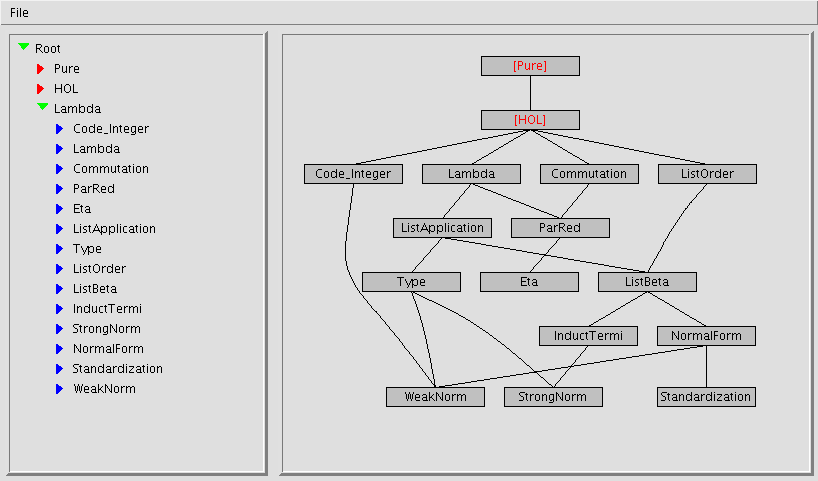
\includegraphics[width=\textwidth]{browser_screenshot}
  \caption{\label{fig:browserwindow} Browser main window}
\end{figure}


\subsubsection*{The directory tree window}

We describe the usage of the directory browser and the meaning of the
different items in the browser window.
\begin{itemize}
  
\item A red arrow before a directory name indicates that the directory
  is currently ``folded'', i.e.~the nodes in this directory are
  collapsed to one single node. In the right sub-window, the names of
  nodes corresponding to folded directories are enclosed in square
  brackets and displayed in red color.
  
\item A green downward arrow before a directory name indicates that
  the directory is currently ``unfolded''. It can be folded by
  clicking on the directory name.  Clicking on the name for a second
  time unfolds the directory again.  Alternatively, a directory can
  also be unfolded by clicking on the corresponding node in the right
  sub-window.
  
\item Blue arrows stand before ordinary node names. When clicking on such a
  name (i.e.\ that of a theory), the graph display window focuses to the
  corresponding node. Double clicking invokes a text viewer window in which
  the contents of the theory file are displayed.

\end{itemize}


\subsubsection*{The graph display window}

When pointing on an ordinary node, an upward and a downward arrow is
shown.  Initially, both of these arrows are green. Clicking on the
upward or downward arrow collapses all predecessor or successor nodes,
respectively. The arrow's color then changes to red, indicating that
the predecessor or successor nodes are currently collapsed. The node
corresponding to the collapsed nodes has the name ``{\tt [....]}''. To
uncollapse the nodes again, simply click on the red arrow or on the
node with the name ``{\tt [....]}''. Similar to the directory browser,
the contents of theory files can be displayed by double clicking on
the corresponding node.


\subsubsection*{The ``File'' menu}

Please note that due to Java security restrictions this menu is not
available in the applet version. The meaning of the menu items is as
follows:
\begin{description}
  
\item[Open \dots] Open a new graph file.
  
\item[Export to PostScript] Outputs the current graph in Postscript format,
  appropriately scaled to fit on one single sheet of A4 paper.  The resulting
  file can be printed directly.
  
\item[Export to EPS] Outputs the current graph in Encapsulated Postscript
  format. The resulting file can be included in other documents.

\item[Quit] Quit the graph browser.

\end{description}


\subsection*{*Syntax of graph definition files}

A graph definition file has the following syntax:
\begin{eqnarray*}
  \mbox{\it graph} & = & \{ \: \mbox{\it vertex \tt ;} \: \} ^ + \\
  vertex & = & \mbox{\it vertexname} \: \mbox{\it vertexID} \: \mbox{\it dirname} \: [ \mbox{\tt +} ]
  \: \mbox{\it path} \: [ \mbox{\tt <} | \mbox{\tt >} ] \: \{ \: \mbox{\it vertexID} \: \} ^ *
\end{eqnarray*}

The meaning of the items in a vertex description is as follows:
\begin{description}
  
\item[vertexname] The name of the vertex.
  
\item[vertexID] The vertex identifier. Note that there may be two
  vertices with equal names, whereas identifiers must be unique.
  
\item[dirname] The name of the ``directory'' the vertex should be
  placed in.  A ``{\tt +}'' sign after {\it dirname} indicates that
  the nodes in the directory are initially visible. Directories are
  initially invisible by default.
  
\item[path] The path of the corresponding theory file. This is
  specified relatively to the path of the graph definition file.
  
\item[List of successor/predecessor nodes] A ``{\tt <}'' sign before
  the list means that successor nodes are listed, a ``{\tt >}'' sign
  means that predecessor nodes are listed. If neither ``{\tt <}'' nor
  ``{\tt >}'' is found, the browser assumes that successor nodes are
  listed.

\end{description}


\section{Creating Isabelle session directories --- \texttt{isatool mkdir}}
\label{sec:tool-mkdir}

The \tooldx{mkdir} utility prepares Isabelle session source directories,
including a sensible default setup of \texttt{IsaMakefile}, \texttt{ROOT.ML},
and a \texttt{document} directory with a minimal \texttt{root.tex} that is
sufficient print all theories of the session (in the order of appearance); see
\S\ref{sec:tool-document} for further information on Isabelle document
preparation.  The usage of \texttt{isatool mkdir} is:
\begin{ttbox}
Usage: mkdir [OPTIONS] [LOGIC] NAME

  Options are:
    -I FILE      alternative IsaMakefile output
    -P           include parent logic target
    -b           setup build mode (session outputs heap image)
    -q           quiet mode

  Prepare session directory, including IsaMakefile and document source,
  with parent LOGIC (default ISABELLE_LOGIC=\$ISABELLE_LOGIC)
\end{ttbox}

The \texttt{mkdir} tool is conservative in the sense that any existing
\texttt{IsaMakefile} etc.\ is left unchanged.  Thus it is safe to invoke it
multiple times, although later runs may not have the desired effect.

Note that \texttt{mkdir} is unable to change \texttt{IsaMakefile}
incrementally --- manual changes are required for multiple sub-sessions.  On
order to get an initial working session, the only editing needed is to add
appropriate \texttt{use_thy} calls to the generated \texttt{ROOT.ML} file.


\subsection*{Options}

The \texttt{-I} option specifies an alternative to \texttt{IsaMakefile} for
dependencies.  Note that ``\texttt{-}'' refers to \emph{stdout}, i.e.\ 
``\texttt{-I-}'' provides an easy way to peek at \texttt{mkdir}'s idea of
\texttt{make} setup required for some particular of Isabelle session.

\medskip The \texttt{-P} option includes a target for the parent
\texttt{LOGIC} session in the generated \texttt{IsaMakefile}.  The
corresponding sources are assumed to be located within the Isabelle
distribution.

\medskip The \texttt{-b} option sets up the current directory as the base for
a new session that provides an actual logic image, as opposed to one that only
runs several theories based on an existing image.  Note that in the latter
case, everything except \texttt{IsaMakefile} would be placed into a separate
directory \texttt{NAME}, rather than the current one.  See
\S\ref{sec:tool-usedir} for further information on \emph{build mode} vs.\ 
\emph{example mode} of the \texttt{usedir} utility.

\medskip The \texttt{-q} enables quiet mode, suppressing further notes on how
to proceed.


\subsection*{Examples}

The standard setup of a single ``example session'' based on the default logic,
with proper document generation is generated like this:
\begin{ttbox}
isatool mkdir Foo && isatool make
\end{ttbox}
\noindent The theory sources should be put into the \texttt{Foo} directory, and its
\texttt{ROOT.ML} should be edited to load all required theories.  Invoking
\texttt{isatool make} again would run the whole session, generating browser
information and the document automatically.  The \texttt{IsaMakefile} is
typically tuned manually later, e.g.\ adding actual source dependencies, or
changing the options passed to \texttt{usedir}.

\medskip Large projects may demand further sessions, potentially with separate
logic images being created.  This usually requires manual editing of the
generated \texttt{IsaMakefile}, which is meant to cover all of the sub-session
directories at the same time (this is the deeper reasong why
\texttt{IsaMakefile} is not made part of the initial session directory created
by \texttt{isatool mkdir}).  See \texttt{src/HOL/IsaMakefile} of the Isabelle
distribution for a full-blown example.


\section{Running Isabelle sessions --- \texttt{isatool usedir}} \label{sec:tool-usedir}

The \tooldx{usedir} utility builds object-logic images, or runs example
sessions based on existing logics. Its usage is:
\begin{ttbox}

Usage: usedir [OPTIONS] LOGIC NAME

  Options are:
    -D PATH      dump generated document sources into PATH
    -P PATH      set path for remote theory browsing information
    -b           build mode (output heap image, using current dir)
    -c BOOL      tell ML system to compress output image (default true)
    -d FORMAT    build document as FORMAT (default false)
    -g BOOL      generate session graph image for document (default false)
    -i BOOL      generate theory browser information (default false)
    -m MODE      add print mode for output
    -p LEVEL     set level of detail for proof objects
    -r           reset session path
    -s NAME      override session NAME
    -v BOOL      be verbose (default false)

  Build object-logic or run examples. Also creates browsing
  information (HTML etc.) according to settings.

  ISABELLE_USEDIR_OPTIONS=
\end{ttbox}

Note that the value of the \settdx{ISABELLE_USEDIR_OPTIONS} setting is
implicitly prefixed to \emph{any} \texttt{usedir} call. Since the
\ttindex{IsaMakefile}s of all object-logics distributed with Isabelle just
invoke \texttt{usedir} for the real work, one may control compilation options
globally via above variable. In particular, generation of \rmindex{HTML}
browsing information and document preparation is controlled here.


\subsection*{Options}

Basically, there are two different modes of operation: \emph{build mode}
(enabled through the \texttt{-b} option) and \emph{example mode} (default).

Calling \texttt{usedir} with \texttt{-b} runs \texttt{isabelle} with input
image \texttt{LOGIC} and output to \texttt{NAME}, as provided on the command
line. This will be a batch session, running \texttt{ROOT.ML} from the current
directory and then quitting.  It is assumed that \texttt{ROOT.ML} contains all
{\ML} commands required to build the logic.

In example mode, \texttt{usedir} runs a read-only session of \texttt{LOGIC}
and automatically runs \texttt{ROOT.ML} from within directory \texttt{NAME}.
It assumes that this file contains appropriate {\ML} commands to run the
desired examples.

\medskip The \texttt{-i} option controls theory browser data generation. It
may be explicitly turned on or off --- as usual, the last occurrence of
\texttt{-i} on the command line wins.

The \texttt{-P} option specifies a path (or actual URL) to be prefixed to any
\emph{non-local} reference of existing theories.  Thus user sessions may
easily link to existing Isabelle libraries already present on the WWW.

The \texttt{-m} options specifies additional print modes to be activated
temporarily while the session is processed.

\medskip The \texttt{-d} option controls document preparation.  Valid
arguments are \texttt{false} (do not prepare any document; this is default),
or any of \texttt{dvi}, \texttt{dvi.gz}, \texttt{ps}, \texttt{ps.gz},
\texttt{pdf}.  The logic session has to provide a properly setup
\texttt{document} directory.  See \S\ref{sec:tool-document} and
\S\ref{sec:tool-latex} for more details.

The \texttt{-g} option produces images of the theory dependency graph (cf.\ 
\S\ref{sec:browse}) for inclusion in the generated document, both as
\texttt{session_graph.eps} and \texttt{session_graph.pdf} at the same time.
In order to make this appear the final {\LaTeX} document one would typically
say \verb,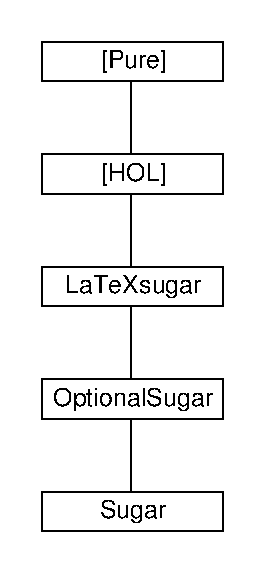
\includegraphics{session_graph}, in the \texttt{document/root.tex}
file.  (Omitting the file-name extension enables {\LaTeX} to select to correct
version, either for the DVI or PDF output path.)

\medskip The \texttt{-D} option causes the generated document sources to be
dumped at location \texttt{PATH}, which is relative to the session's main
directory.  For example, \texttt{-D document} would leave a copy of the
{\LaTeX} sources in the actual document directory.  Thus the Isabelle
\texttt{document} or \texttt{latex} tools may be run later, facilitating much
easier debugging of {\LaTeX} errors, for example.  A copy of the Isabelle
style files will be placed in \texttt{PATH} as well.

\medskip The \texttt{-p} option determines the level of detail for internal
proof objects, see also the \emph{Isabelle Reference
  Manual}~\cite{isabelle-ref}.

\medskip The \texttt{-v} option causes additional information to be printed
during while running the session, notably the location of prepared documents.

\medskip Any \texttt{usedir} session is named by some \emph{session
  identifier}. These accumulate, documenting the way sessions depend on
others. For example, consider \texttt{Pure/FOL/ex}, which refers to the
examples of FOL, which in turn is built upon Pure.

The current session's identifier is by default just the base name of the
\texttt{LOGIC} argument (in build mode), or of the \texttt{NAME} argument (in
example mode). This may be overridden explicitly via the \texttt{-s} option.


\subsection*{Examples}

Refer to the \texttt{IsaMakefile}s of the Isabelle distribution's
object-logics as a model for your own developments.  For example, see
\texttt{src/FOL/IsaMakefile}.  The Isabelle \texttt{mkdir} tool (see
\S\ref{sec:tool-mkdir}) creates \texttt{IsaMakefile}s with proper invocation
of \texttt{usedir} as well.


\section{Preparing Isabelle session documents --- \texttt{isatool document}}
\label{sec:tool-document}

The \tooldx{document} utility prepares logic session documents, processing the
sources both as provided by the user and generated by Isabelle.  Its usage is:
\begin{ttbox}
Usage: document [OPTIONS] [DIR]

  Options are:
    -c           cleanup -- be aggressive in removing old stuff
    -o FORMAT    specify output format: dvi (default), dvi.gz, ps,
                 ps.gz, pdf

  Prepare the theory session document in DIR (default 'document')
  producing the specified output format.
\end{ttbox}
This tool is usually run automatically as part of the corresponding Isabelle
batch process, provided document preparation has been enabled (cf.\ the
\texttt{-d} option of the \texttt{usedir} utility, \S\ref{sec:tool-usedir}).
It may be manually invoked on the generated browser information document
output as well, e.g.\ in case of errors encountered in the batch run.

\medskip Document preparation requires a properly setup ``\texttt{document}''
directory within the logic session sources.  This directory is supposed to
contain all the files needed to produce the final document --- apart from the
actual theories which are generated by Isabelle.

\medskip For most practical purposes, the \texttt{document} tool is smart
enough to create any of the specified output formats, taking \texttt{root.tex}
supplied by the user as a starting point.  This even includes multiple runs of
{\LaTeX} to accommodate references and bibliographies (the latter assumes
\texttt{root.bib} within the same directory).

In more complex situations, a separate \texttt{IsaMakefile} for the document
sources may be given instead.  This should provide targets for any admissible
document format; these have to produce corresponding output files named after
\texttt{root} as well, e.g.\ \texttt{root.dvi} for target format \texttt{dvi}.

\medskip When running the session, Isabelle copies the original
\texttt{document} directory into its proper place within
\texttt{ISABELLE_BROWSER_INFO} according to the session path.  Then, for any
processed theory $A$ some {\LaTeX} source is generated and put there as
$A$\texttt{.tex}.  Furthermore, a list of all generated theory files is put
into \texttt{session.tex}.  Typically, the root {\LaTeX} file provided by the
user would include \texttt{session.tex} to get a document containing all the
theories.

The {\LaTeX} versions of the theories require some macros defined in
\texttt{isabelle.sty} as distributed with Isabelle.  Doing
\verb,\usepackage{isabelle}, somewhere in \texttt{root.tex} should work fine;
the underlying Isabelle \texttt{latex} utility already includes an appropriate
{\TeX} inputs path.

If the text contains any references to Isabelle symbols (such as
\verb,\<forall>,) then \texttt{isabellesym.sty} should be included as well.
This package contains a standard set of {\LaTeX} macro definitions
\verb,\isasym,$foo$ corresponding to \verb,\<,$foo$\verb,>, (see
Appendix~\ref{app:symbols} for a complete list of predefined Isabelle
symbols).  Users may invent further symbols as well, just by providing
{\LaTeX} macros in a similar fashion as in \texttt{isabellesym.sty} of the
distribution.

For proper setup of PDF documents (with hyperlinks, bookmarks, and thumbnail
images), we recommend to include \verb,pdfsetup.sty, as well.  It is safe to
do so even without using PDF~\LaTeX.

\medskip As a final step of document preparation within Isabelle,
\texttt{isatool document -c} is run on the resulting \texttt{document}
directory.  Thus the actual output document is built and installed in its
proper place (as linked by the session's \texttt{index.html} if option
\texttt{-i} of \texttt{usedir} has been enabled, cf.\ \S\ref{sec:info}).  The
generated sources are deleted after successful run of {\LaTeX} and friends.
Note that a separate copy of the sources may be retained by passing an option
\texttt{-D} to the \texttt{usedir} utility when running the session (see also
\S\ref{sec:tool-usedir}).


\section{Running {\LaTeX} within the Isabelle environment --- \texttt{isatool latex}}
\label{sec:tool-latex}

The \tooldx{latex} utility provides the basic interface for Isabelle document
preparation.  Its usage is:
\begin{ttbox}
Usage: latex [OPTIONS] [FILE]

  Options are:
    -o FORMAT    specify output format: dvi (default), dvi.gz, ps,
                 ps.gz, pdf, bbl, png, sty

  Run LaTeX (and related tools) on FILE (default root.tex),
  producing the specified output format.
\end{ttbox}
Appropriate {\LaTeX}-related programs are run on the input file, according to
the given output format: \texttt{latex}, \texttt{pdflatex}, \texttt{dvips},
\texttt{bibtex} (for \texttt{bbl}), and \texttt{thumbpdf} (for \texttt{png}).
The actual commands are determined from the settings environment
(\texttt{ISABELLE_LATEX} etc., see \S\ref{sec:settings}).

The \texttt{sty} output format causes the Isabelle style files to be updated
from the distribution.  This is useful in special situations where the
document sources are to be processed another time by separate tools (cf.\ 
option \texttt{-D} of the \texttt{usedir} utility, see
\S\ref{sec:tool-usedir}).


\subsubsection*{Examples}

Invoking \texttt{isatool latex} by hand may be occasionally useful when
debugging failed attempts of the automatic document preparation stage of
batch-mode Isabelle.  The abortive process leaves the sources at a certain
place within \texttt{ISABELLE_BROWSER_INFO}, see the runtime error message for
details.  This enables users to inspect {\LaTeX} runs in further detail, e.g.\ 
like this:

\begin{ttbox}
  cd ~/isabelle/browser_info/HOL/Test/document
  isatool latex -o pdf
\end{ttbox}


%%% Local Variables: 
%%% mode: latex
%%% TeX-master: "system"
%%% End: 


% $Id$

\chapter{Miscellaneous tools} \label{ch:tools}

Subsequently we describe various Isabelle related utilities, given in
alphabetical order.


\section{Converting legacy ML scripts --- \texttt{isatool convert}}

The \tooldx{convert} utility assists in converting legacy ML proof scripts
into the new-style format of Isabelle/Isar:
\begin{ttbox}
Usage: convert [FILES|DIRS...]

  Recursively find .ML files, converting legacy tactic scripts to
  Isabelle/Isar tactic emulation.
  Note: conversion is only approximated, based on some heuristics.

  Renames old versions of FILES by appending "~0~".
  Creates new versions of FILES by appending ".thy".
\end{ttbox}
The resulting theory text uses the tactic emulation facilities of
Isabelle/Isar (see also \cite{isabelle-ref}, especially the ``Conversion
guide'' in the appendix).  Usually there is some manual tuning required to get
an automatically converted script work again --- the success rate is around
99\% for common ML scripts.


\section{Displaying documents --- \texttt{isatool display}}

The \tooldx{display} utility displays documents in DVI format:
\begin{ttbox}
Usage: display [OPTIONS] FILE

  Options are:
    -c           cleanup -- remove FILE after use

  Display document FILE (in DVI format).
\end{ttbox}

\medskip The \texttt{-c} option causes the input file to be removed after use.
The program for viewing \texttt{dvi} files is determined by the
\texttt{DVI_VIEWER} setting.


\section{Viewing documentation --- \texttt{isatool doc}} \label{sec:tool-doc}

The \tooldx{doc} utility displays online documentation:
\begin{ttbox}
Usage: doc [DOC]

  View Isabelle documentation DOC, or show list of available documents.
\end{ttbox}
If called without arguments, it lists all available documents. Each line
starts with an identifier, followed by a short description. Any of these
identifiers may be specified as the first argument in order to have the
corresponding document displayed.

\medskip The \texttt{ISABELLE_DOCS} setting specifies the list of directories
(separated by colons) to be scanned for documentations.  The program for
viewing \texttt{dvi} files is determined by the \texttt{DVI_VIEWER} setting.


\section{Tuning proof scripts --- \texttt{isatool expandshort}}

The \tooldx{expandshort} utility tunes {\ML} proof scripts to enhance
readability:
\begin{ttbox}
Usage: expandshort [FILES|DIRS...]

  Recursively find .ML files, expand shorthand goal commands.  Also
  contracts uses of resolve_tac, dresolve_tac, eresolve_tac,
  forward_tac, rewrite_goals_tac on 1-element lists; furthermore
  expands tabs, which are forbidden in SML string constants.

  Renames old versions of files by appending "~~".
\end{ttbox}
In the files or directories supplied as arguments, all occurrences of the
shorthand commands \texttt{br}, \texttt{be} etc.\ in proof scripts are
replaced with the corresponding full commands.  The old versions of the files
are renamed to have the suffix ``\verb'~~'''.


\section{Getting logic images --- \texttt{isatool findlogics}}

The \tooldx{findlogics} utility traverses all directories specified in
\texttt{ISABELLE_PATH}, looking for Isabelle logic images. Its usage is:
\begin{ttbox}
Usage: findlogics

  Collect heap file names from ISABELLE_PATH.
\end{ttbox}
The base names of all files found on the path are printed --- sorted and with
duplicates removed. Also note that lookup in \texttt{ISABELLE_PATH} includes
the current values of \texttt{ML_SYSTEM} and \texttt{ML_PLATFORM}. Thus
switching to another {\ML} compiler may change the set of logic images
available.


\section{Inspecting the settings environment --- \texttt{isatool getenv}}
\label{sec:tool-getenv}

The Isabelle settings environment --- as provided by the site-default and
user-specific settings files --- can be inspected with the \tooldx{getenv}
utility:
\begin{ttbox}
Usage: getenv [OPTIONS] [VARNAMES ...]

  Options are:
    -a           display complete environment
    -b           print values only (doesn't work for -a)

  Get value of VARNAMES from the Isabelle settings.
\end{ttbox}

With the \texttt{-a} option, one may inspect the full process environment that
Isabelle related programs are run in. This usually contains much more
variables than are actually Isabelle settings.  Normally, output is a list of
lines of the form \mbox{$name$\texttt{=}$value$}. The \texttt{-b} option
causes only the values to be printed.


\subsection*{Examples}

Get the {\ML} system name and the location where the compiler binaries are
supposed to reside as follows:
\begin{ttbox}
isatool getenv ML_SYSTEM ML_HOME
{\out ML_SYSTEM=polyml}
{\out ML_HOME=/usr/share/polyml/x86-linux}
\end{ttbox}

The next one peeks at the output directory for \texttt{isabelle} logic images:
\begin{ttbox}
isatool getenv -b ISABELLE_OUTPUT
{\out /home/me/isabelle/heaps/polyml_x86-linux}
\end{ttbox}
Here we have used the \texttt{-b} option to suppress the
\texttt{ISABELLE_OUTPUT=} prefix.  The value above is what became of the
following assignment in the default settings file:
\begin{ttbox}
ISABELLE_OUTPUT="\$ISABELLE_HOME_USER/heaps"
\end{ttbox}
Note how the \texttt{ML_IDENTIFIER} value got appended automatically to each
path component. This is a special feature of \texttt{ISABELLE_OUTPUT}.


\section{Installing standalone Isabelle executables --- \texttt{isatool install}}
\label{sec:tool-install}

By default, the Isabelle binaries (\texttt{isabelle}, \texttt{isatool} etc.)
are just run from their location within the distribution directory, probably
indirectly by the shell through its \texttt{PATH}.  Other schemes of
installation are supported by the \tooldx{install} utility:
\begin{ttbox}
Usage: install [OPTIONS]

  Options are:
    -d DISTDIR   use DISTDIR as Isabelle distribution
                 (default ISABELLE_HOME)
    -p DIR       install standalone binaries in DIR

  Install Isabelle executables with absolute references to the current
  distribution directory.
\end{ttbox}

The \texttt{-d} option overrides the current Isabelle distribution directory
as determined by \texttt{ISABELLE_HOME}.

The \texttt{-p} option installs executable wrapper scripts for
\texttt{isabelle}, \texttt{isatool}, \texttt{Isabelle}, containing proper
absolute references to the Isabelle distribution directory.  A typical
\texttt{DIR} specification would be some directory expected to be in the
shell's \texttt{PATH}, such as \texttt{/usr/local/bin}.  It is important to
note that a plain manual copy of the original Isabelle executables just would
not work!


\section{Creating instances of the Isabelle logo --- \texttt{isatool
    logo}}

The \tooldx{logo} utility creates any instance of the generic Isabelle logo as
an Encapsuled Postscript file (EPS):
\begin{ttbox}
Usage: logo [OPTIONS] NAME

  Create instance NAME of the Isabelle logo (as EPS).

  Options are:
    -o OUTFILE   set output file (default determined from NAME)
    -q           quiet mode
\end{ttbox}
You are encouraged to use this to create a derived logo for your Isabelle
project.  For example, \texttt{isatool logo Bali} creates
\texttt{isabelle_bali.eps}.


\section{Isabelle's version of make --- \texttt{isatool make}}
\label{sec:tool-make}

The Isabelle \tooldx{make} utility is a very simple wrapper for
ordinary Unix \texttt{make}:
\begin{ttbox}
Usage: make [ARGS ...]

  Compile the logic in current directory using IsaMakefile.
  ARGS are directly passed to the system make program.
\end{ttbox}
Note that the Isabelle settings environment is also active. Thus one
may refer to its values within the \ttindex{IsaMakefile}, e.g.\ 
\texttt{\$(ISABELLE_OUTPUT)}. Furthermore, programs started from the
make file also inherit this environment.  Typically,
\texttt{IsaMakefile}s defer the real work to the \texttt{usedir}
utility, see \S\ref{sec:tool-usedir}.

\medskip The basic \texttt{IsaMakefile} convention is that the default
target builds the actual logic, including its parents if appropriate.
The \texttt{images} target is intended to build all local logic
images, while the \texttt{test} target shall build all related
examples.  The \texttt{all} target shall do \texttt{images} and
\texttt{test}.


\subsection*{Examples}

Refer to the \texttt{IsaMakefile}s of the Isabelle distribution's
object-logics as a model for your own developments.  For example, see
\texttt{src/FOL/IsaMakefile}.


\section{Make all logics --- \texttt{isatool makeall}}

The \tooldx{makeall} utility applies Isabelle make to all logic
directories of the distribution:
\begin{ttbox}
Usage: makeall [ARGS ...]

  Apply isatool make to all logics (passing ARGS).
\end{ttbox}
The arguments \texttt{ARGS} are just passed verbatim to each
\texttt{make} invocation.


\section{Printing documents --- \texttt{isatool print}}

The \tooldx{print} utility prints documents:
\begin{ttbox}
Usage: print [OPTIONS] FILE

  Options are:
    -c           cleanup -- remove FILE after use

  Print document FILE.
\end{ttbox}

The \texttt{-c} option causes the input file to be removed after use.  The
printer spool command is determined by the \texttt{PRINT_COMMAND} setting.


\section{Remove awkward symbol names from theory sources --- \texttt{isatool unsymbolize}}

The \tooldx{unsymbolize} utility tunes Isabelle theory sources to improve
readability for plain ASCII output (e.g.\ in email communication).  Most
notably, \texttt{unsymbolize} replaces awkward arrow symbols such as
\verb|\<Longrightarrow>| by \verb|==>|.
\begin{ttbox}
Usage: unsymbolize [FILES|DIRS...]

  Recursively find .thy/.ML files, removing unreadable symbol names.
  Note: this is an ad-hoc script; there is no systematic way to replace
  symbols independently of the inner syntax of a theory!

  Renames old versions of FILES by appending "~~".
\end{ttbox}


\section{Output the version identifier of the Isabelle distribution --- \texttt{isatool version}}

The \tooldx{version} utility outputs the full version string of the
Isabelle distribution being used, e.g.\ ``\texttt{Isabelle2007:
  November 2007}''.  There are no options nor arguments.

%%% Local Variables: 
%%% mode: latex
%%% TeX-master: "system"
%%% End: 


\chapter{Fonts and character encodings}

With the advent of print modes in Isabelle, variant forms of output
have become very easy. As the canonical application of this feature,
{\Pure} and major object-logics (\FOL, \ZF, \HOL, \HOLCF) support
optional input and output of nice mathematical symbols as an built-in
option.

Symbolic output is enabled by activating the \ttindex{symbols} print
mode. User interfaces (e.g.\ \texttt{isa-xterm}, see
\S\ref{sec:interface}) usually do this already by default.

\medskip Displaying non-standard characters requires special screen
fonts, of course. The \texttt{installfonts} utility takes care of
this, see \S\ref{sec:tool-installfonts}. Furthermore, some {\ML}
systems disallow non-\textsc{ascii} characters in literal strings.
This problem is avoided by the \texttt{symbolinput} filter (see
\S\ref{sec:tool-symbolinput}).

Both of these are invoked transparently in normal operation. So one
does not actually have to read the explanations below, unless
something fails to work.


\section{Telling X11 about the Isabelle fonts --- \texttt{isatool installfonts}}
\label{sec:tool-installfonts}

The \tooldx{installfonts} utility ensures that your currently running
X11 display server (as determined by the \texttt{DISPLAY} environment
variable) knows about the Isabelle fonts. Its usage is:
\begin{ttbox}
Usage: isatool installfonts

  Install the isabelle fonts into your X11 server.
  (May be safely called repeatedly.)
\end{ttbox}
Note that this need not be called manually under normal circumstances
--- user interfaces depending on the Isabelle fonts usually invoke
\texttt{installfonts} automatically.

\medskip As simple as this might appear to be, it is not! X11 fonts
are a surprisingly complicated matter. Depending on your network
structure, fonts might have to be installed differently. This has to
be specified via the \settdx{ISABELLE_INSTALLFONTS} variable in your
local settings.

\medskip In the simplest situation, X11 is used only locally, i.e.\ 
the client program (Isabelle) and the display server are run on the
same machine. In this case, most X11 display servers should be happy
by being told about the Isabelle fonts directory as follows:
\begin{ttbox}
ISABELLE_INSTALLFONTS="xset fp+{\thinspace}$ISABELLE_HOME/lib/fonts; xset fp rehash"
\end{ttbox}
The same also works for remote X11 sessions in a somewhat homogeneous
network, where the X11 display machine mounts the Isabelle
distribution under the same name as the client side.

\medskip Above method fails, though, if the display machine does have
the font files at the same location as the client. In case your server
is a full workstation with its own file system, you could in principle
just copy the fonts there and do an appropriate \texttt{xset~fp+}
manually before running the Isabelle interface. This is very awkward,
of course. It is even \emph{impossible} for proper X terminals that do
not have their own file system.

A much better solution is to have a \emph{font server} offer the
Isabelle fonts to any X display on the network.  There is already a
suitable server running at Munich. So in case you have a sensible
Internet connection, you may just attach yourself as follows:
\begin{ttbox}
ISABELLE_INSTALLFONTS="xset fp+ tcp/isafonts.informatik.tu-muenchen.de:7200"
\end{ttbox}

\medskip In the unfortunate case that neither local fonts work, nor
accessing our world-wide font service is practical, it might be best
to start your own in-house font service. This is in principle easy to
setup. The program is called \texttt{xfs} (or just \texttt{fs)}, see
the \texttt{man} pages of your system. There is an example
configuration available in the \texttt{lib/fontserver} directory of
the Isabelle distribution.



\section{Filtering non-ASCII characters --- \texttt{isatool symbolinput}}
\label{sec:tool-symbolinput}

Processing non-\textsc{ascii} text is notoriously difficult.  In
particular, some {\ML} systems reject character codes outside the
range 32--127 as part of literal string constants. In order to
circumvent such restrictions, Isabelle employs a general notation
where glyphs are referred by some symbolic name instead of their
actual encoding: Its general form is \verb|\<|$charname$\verb|>|.

The \tooldx{symbolinput} utility converts a input stream encoded
according to the standard Isabelle font layout into pure
\textsc{ascii} text. There is no usage --- \texttt{symbolinput} just
works from standard input to standard output, without any options
available.

\medskip For example, the non-\textsc{ascii} input string \texttt{"A
  $\land$ B $\lor$ C"} will be replaced by \verb|"A \\<and> B \\<or> C"|.
Note that the \verb|\| are escaped, accomodating concrete {\ML} string
syntax.

\medskip In many cases, it might be wise not to rely on symbolic
characters and avoid non-\textsc{ascii} text in files altogether. Then
symbolic syntax would be really optional, with always suitable
\textsc{ascii} representations available: In theory definitions
symbols appear only in mixfix annotations --- using the
\verb|\<|$charname$\verb|>| form, proof scripts are just left in plain
\textsc{ascii}.

Thus users with \textsc{ascii}-only facilities will still be able to
read your files.


%FIXME not yet
%\section{ --- \texttt{isatool showsymbols}}
%
%\begin{ttbox}
%\end{ttbox}


\appendix
\let\int\intorig

% $Id$

\chapter{Isabelle symbols}\label{app:symbols}

Isabelle supports an infinite number of non-ASCII symbols, which are
represented in source text as \verb,\<,$name$\verb,>, (where $name$ may be any
identifier).  It is left to front-end tools how these symbols are presented to
the user.  The following predefined standard symbols are available by default
for Isabelle document output; they are also supported by Proof~General when
used together with the X-Symbol package.

\begin{center}
  \input{syms}  
\end{center}

Any symbol (or plain ASCII character) may be prefixed by a control sequence
\verb,\<^sup>, for superscript and \verb,\<^sub>, for subscript.  E.g.\ 
\verb,A\<^sup>\<star>, is presented in {\LaTeX} as
\isa{A\isactrlsup{\isasymstar}}.  See also Chapter~\ref{ch:present} for more
information on Isabelle document preparation and related issues.

%%% Local Variables: 
%%% mode: latex
%%% TeX-master: "system"
%%% End: 


\begingroup
  \bibliographystyle{plain} \small\raggedright\frenchspacing
  \bibliography{../manual}
\endgroup

\printindex

\end{document}
